\documentclass{standalone}
\usepackage{tikz,amsmath}
\usepackage{tkz-euclide}
\begin{document}
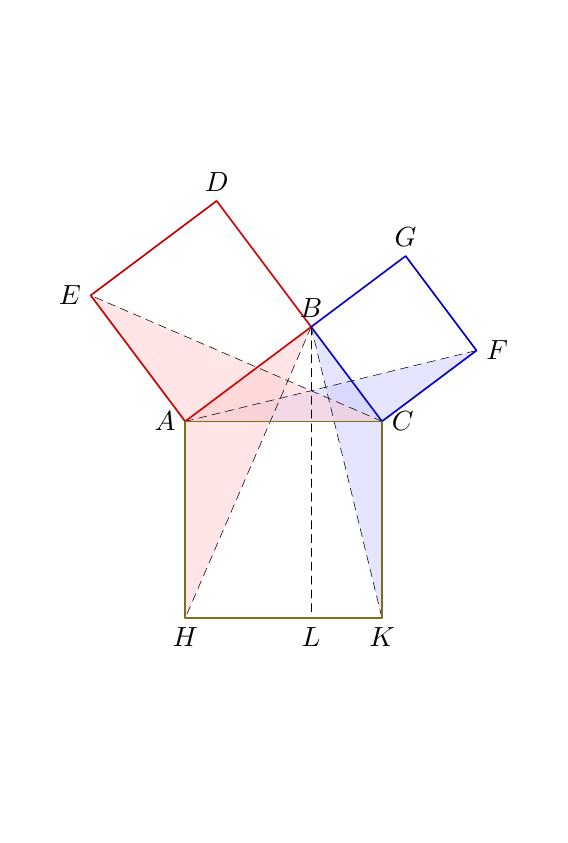
\begin{tikzpicture}[>=latex, scale=1]
  \useasboundingbox(-2,-5)rectangle(4.5,5);
  \tkzDefPoints{0/0/A,2.5/0/C,1.6/1.2/B}
  \tkzDefPointWith[orthogonal,K=-1](A,C)\tkzGetPoint{H}
  \tkzDefPointWith[orthogonal,K=1](C,A)\tkzGetPoint{K}
  \tkzDefPointWith[orthogonal,K=1](A,B)\tkzGetPoint{E}
  \tkzDefPointWith[orthogonal,K=-1](B,A)\tkzGetPoint{D}
  \tkzDefPointWith[orthogonal,K=-1](C,B)\tkzGetPoint{F}
  \tkzDefPointWith[orthogonal,K=1](B,C)\tkzGetPoint{G}
  \tkzDefPointBy[projection = onto H--K](B)\tkzGetPoint{L}
  \tkzFillPolygon[opacity=0.5,fill=blue!20!white](A,F,C)
  \tkzFillPolygon[opacity=0.5,fill=blue!20!white](B,C,K)
  \tkzFillPolygon[opacity=0.5,fill=red!20!white](A,E,C)
  \tkzFillPolygon[opacity=0.5,fill=red!20!white](B,A,H)
  \tkzDrawSegments[densely dashed](C,E A,F B,H B,K B,L)
  \tkzDrawPolygon[semithick,red!80!black](A,B,D,E)
  \tkzDrawPolygon[semithick,blue!80!black](C,B,G,F)
  \tkzDrawPolygon[semithick,olive!80!black](C,A,H,K)
  \tkzLabelPoints(H,K,L)
  \tkzLabelPoints[above](B,G,D)
  \tkzLabelPoints[left](A,E)
  \tkzLabelPoints[right](C,F)
\end{tikzpicture}
\end{document}